%% FullCourse_10Lecs -- Lecture 3, Topic 3.2: Neural Network Concepts
%% Source: ./archive_pre_split/Lec03_ML_for_Macro.tex (section 3)
%% Pass B: layer in refinements from
%%         ../../MiniCourse_8hr/Slides/Module1_ML_Foundations/M1_T2_NN_Concepts.tex

%% Shared preamble for the FullCourse_10Lecs topic decks.
%%
%% Each topic .tex \input's this file, then defines its own \title, \date
%% override (if any), \graphicspath, and \begin{document}.
%%
%% Reconstructed verbatim from the inlined copy preserved in
%% Lec10_Case_Studies/Lec10_T8_Case6_DeepRamsey.tex (lines 23-190), which is
%% explicitly annotated there as "from ../shared_preamble.tex, copied verbatim".
%% Base preamble matches MiniCourse_8hr/Slides/shared_preamble.tex; this version
%% additionally provides \sectiondivider, the conceptbox/cautionbox/examplebox/
%% takeawaybox tcolorboxes, and \compacttables used across the split decks.

\documentclass[10pt,english,aspectratio=169]{beamer}

\usepackage{ae,aecompl}
\usepackage[T1]{fontenc}
\usepackage{textcomp}
\usepackage[utf8]{inputenc}
\usepackage{babel}
\usepackage{datetime2}

\setcounter{secnumdepth}{3}
\setcounter{tocdepth}{3}

\usepackage{amsmath, amssymb, amsthm, graphicx}
\usepackage{booktabs, multirow}
\usepackage{tikz}
\usepackage{pgfplots}
\pgfplotsset{compat=1.16}
\usepackage[most]{tcolorbox}
\tcbuselibrary{skins, breakable, theorems}
\usepackage{listings}
\usepackage{xcolor}

\lstset{
  basicstyle=\ttfamily\small,
  keywordstyle=\color{blue!80!black}\bfseries,
  commentstyle=\color{green!50!black}\itshape,
  stringstyle=\color{orange!80!black},
  backgroundcolor=\color{gray!8},
  frame=single,
  rulecolor=\color{gray!40},
  breaklines=true,
  showstringspaces=false,
  numbers=none,
}

\lstdefinestyle{pythonstyle}{
    language=Python,
    basicstyle=\ttfamily\footnotesize,
    keywordstyle=\color{blue!80!black}\bfseries,
    commentstyle=\color{green!50!black}\itshape,
    stringstyle=\color{orange!80!black},
    frame=single,
    breaklines=true,
    showstringspaces=false,
    numbers=left,
    numbersep=5pt,
    numberstyle=\tiny\color{gray},
    backgroundcolor=\color{gray!8},
    rulecolor=\color{gray!40}
}

\ifx\hypersetup\undefined
  \AtBeginDocument{%
    \hypersetup{bookmarks=false,breaklinks=true,pdfborder={0 0 0},colorlinks=true,
      linkcolor=DarkText,urlcolor=RedTitle}%
  }
\else
  \hypersetup{bookmarks=false,breaklinks=true,pdfborder={0 0 0},colorlinks=true,
    linkcolor=DarkText,urlcolor=RedTitle}%
\fi

\makeatletter
\newcommand\makebeamertitle{%
  \begin{frame}[plain]
    \vspace*{1.0cm}
    \centering
    {\usebeamerfont{title}\usebeamercolor[fg]{title}\inserttitle\par}
    \vspace{1.0cm}
    {\usebeamerfont{author}\usebeamercolor[fg]{author}\insertauthor\par}
    \vspace{0.2cm}
    {\usebeamerfont{date}\usebeamercolor[fg]{date}\insertdate\par}
  \end{frame}}%
\AtBeginDocument{%
  \let\origtableofcontents=\tableofcontents
  \def\tableofcontents{\@ifnextchar[{\origtableofcontents}{\gobbletableofcontents}}
  \def\gobbletableofcontents#1{\origtableofcontents}%
}

\usetheme{metropolis}
\usefonttheme{professionalfonts}

\definecolor{LightGray}{RGB}{230,230,230}
\definecolor{RedTitle}{RGB}{0,0,200}
\definecolor{VeryLightGray}{RGB}{245,245,245}
\definecolor{DarkText}{RGB}{0,0,0}

\setbeamercolor{background canvas}{bg=white}
\setbeamercolor{title}{fg=RedTitle}
\setbeamercolor{author}{fg=DarkText}
\setbeamercolor{date}{fg=DarkText}
\setbeamercolor{frametitle}{bg=VeryLightGray,fg=DarkText}
\setbeamercolor{normal text}{fg=DarkText}
\setbeamerfont{title}{size=\large}

\setbeamersize{text margin left=5mm, text margin right=5mm}
\addtobeamertemplate{frametitle}{}{\vspace{-0.5em}}
\newcommand{\reducevspace}{\vspace{-0.5cm}}

% Shared section divider and box styles for split topic decks.
\newcommand{\sectiondivider}[2]{%
\begin{frame}[plain,noframenumbering]
\begin{center}
\vfill
{\Large\textbf{#1}\par}
\vspace{0.35cm}
{\normalsize #2\par}
\vfill
\end{center}
\end{frame}
}

\newtcolorbox{conceptbox}[1][]{
  colback=blue!3,
  colframe=RedTitle!55,
  boxrule=0.35mm,
  arc=1mm,
  left=2mm,
  right=2mm,
  top=1mm,
  bottom=1mm,
  #1
}
\newtcolorbox{cautionbox}[1][]{
  colback=red!3,
  colframe=red!50!black,
  boxrule=0.35mm,
  arc=1mm,
  left=2mm,
  right=2mm,
  top=1mm,
  bottom=1mm,
  #1
}
\newtcolorbox{examplebox}[1][]{
  colback=green!3,
  colframe=green!45!black,
  boxrule=0.35mm,
  arc=1mm,
  left=2mm,
  right=2mm,
  top=1mm,
  bottom=1mm,
  #1
}
\newtcolorbox{takeawaybox}[1][]{
  colback=VeryLightGray,
  colframe=RedTitle!55,
  boxrule=0.35mm,
  arc=1mm,
  left=2mm,
  right=2mm,
  top=1mm,
  bottom=1mm,
  #1
}
\newcommand{\compacttables}{\renewcommand{\arraystretch}{1.15}}

\setbeamertemplate{navigation symbols}{}
\setbeamertemplate{footline}{%
  \hfill%
  \usebeamercolor[fg]{page number in head/foot}%
  \usebeamerfont{page number in head/foot}%
  \insertframenumber\,/\,\inserttotalframenumber\kern1em\vskip2pt%
}

\makeatother

\author{Zhigang Feng}
% "date with time": compile timestamp so each build is identifiable.
\date{\today\ \DTMcurrenttime}


\graphicspath{{./pic/}{../../MiniCourse_8hr/Slides/Module1_ML_Foundations/pic/}{../}}

% Suppress the redundant auto-generated metropolis section page; the
% \sectiondivider frames below are the dividers we keep.
\metroset{sectionpage=none}
\usetikzlibrary{positioning,arrows.meta,shapes,calc}
%% Lec03 shared MAP slide: "one map, four acts" recurring diagram.
%% Input this file AFTER ../shared_preamble.tex (needs RedTitle, VeryLightGray,
%% DarkText) and AFTER \usetikzlibrary{positioning,arrows.meta,shapes,calc}.
%% Call \LecThreeMap{k} inside a frame, where k in {1,2,3,4} highlights the
%% current act ("you are here") and k = 0 renders the closing reprise with all
%% four acts checked green (used by T4's closing frame).
%% Filename deliberately does NOT match the build glob Lec*_T*.tex, so the build
%% script never tries to compile it standalone.
%%
%% The four acts are the lecture's story: WHY -> BUILD -> TRAIN -> SHAPE, i.e.
%% the case for ML in economics, the network as an object (architecture + UAT),
%% the learning machinery (backprop + SGD + regularization + double descent),
%% and economics-aware architectures with the hands-on lab.

\newcommand{\LecThreeMap}[1]{%
% Precompute per-box style selectors; TikZ option lists are comma-split before
% TeX conditionals run, so \ifnum must not sit inside a [...] options list.
\ifnum#1=0
  \tikzset{lmapa/.style={lmapdone}, lmapb/.style={lmapdone},
           lmapc/.style={lmapdone}, lmapd/.style={lmapdone}}%
\else
  \tikzset{lmapa/.style={}, lmapb/.style={}, lmapc/.style={}, lmapd/.style={}}%
  \ifnum#1=1 \tikzset{lmapa/.style={lmapcur}}\fi
  \ifnum#1=2 \tikzset{lmapb/.style={lmapcur}}\fi
  \ifnum#1=3 \tikzset{lmapc/.style={lmapcur}}\fi
  \ifnum#1=4 \tikzset{lmapd/.style={lmapcur}}\fi
\fi
\begin{center}
\begin{tikzpicture}[
    act/.style={rectangle, rounded corners, draw=black!60, fill=VeryLightGray,
        minimum width=3.0cm, minimum height=0.95cm, text width=2.9cm,
        align=center, font=\small, text=DarkText},
    lmapcur/.style={draw=RedTitle, very thick, fill=orange!20},
    lmapdone/.style={draw=green!45!black, thick, fill=green!10},
    q/.style={font=\tiny\itshape, text width=3.0cm, align=center, text=black!70},
    barlab/.style={font=\tiny\bfseries, text=black!65},
    sat/.style={rectangle, rounded corners, draw=black!45, dashed, fill=white,
        text width=5.2cm, align=center, font=\tiny, text=black!70,
        minimum height=0.5cm},
    arr/.style={-{Stealth[length=2.2mm]}, thick, gray!60}
]
    % --- four act boxes ---
    \node[act, lmapa] (a1) at (0,0)
        {\textbf{3.1\ \ WHY}\\[1pt] \tiny the case for ML in econ};
    \node[act, lmapb] (a2) at (3.6,0)
        {\textbf{3.2\ \ BUILD}\\[1pt] \tiny neurons $\cdot$ activations $\cdot$ UAT};
    \node[act, lmapc] (a3) at (7.2,0)
        {\textbf{3.3\ \ TRAIN}\\[1pt] \tiny backprop $\cdot$ SGD $\cdot$ dbl.\ descent};
    \node[act, lmapd] (a4) at (10.8,0)
        {\textbf{3.4\ \ SHAPE}\\[1pt] \tiny ICNN $\cdot$ monotone $\cdot$ lab};
    \draw[arr] (a1) -- (a2);
    \draw[arr] (a2) -- (a3);
    \draw[arr] (a3) -- (a4);
    % --- the student question each act answers ---
    \node[q] at (0,-0.95)    {why should an economist\\ care about ML?};
    \node[q] at (3.6,-0.95)  {what is a neural network,\\ and why does it work?};
    \node[q] at (7.2,-0.95)  {how does it learn ---\\ and why not overfit?};
    \node[q] at (10.8,-0.95) {how do I build economics\\ in --- and run it myself?};
    % --- "you are here" marker above the current act ---
    \ifnum#1=1 \node[font=\scriptsize\bfseries, text=RedTitle] at (0,0.98)
        {you are here\ $\blacktriangledown$};\fi
    \ifnum#1=2 \node[font=\scriptsize\bfseries, text=RedTitle] at (3.6,0.98)
        {you are here\ $\blacktriangledown$};\fi
    \ifnum#1=3 \node[font=\scriptsize\bfseries, text=RedTitle] at (7.2,0.98)
        {you are here\ $\blacktriangledown$};\fi
    \ifnum#1=4 \node[font=\scriptsize\bfseries, text=RedTitle] at (10.8,0.98)
        {you are here\ $\blacktriangledown$};\fi
    \ifnum#1=0 \node[font=\scriptsize\bfseries, text=green!45!black] at (5.4,0.98)
        {all four acts complete};\fi
    % --- bottom band: the ML pipeline (the technical spine of the lecture) ---
    \fill[blue!10]   (-1.55,-1.72) rectangle (5.15,-1.40);
    \fill[green!12]  (5.65,-1.72)  rectangle (8.75,-1.40);
    \fill[orange!16] (9.25,-1.72)  rectangle (12.35,-1.40);
    \node[barlab] at (1.8,-1.56)  {REPRESENT\ (UAT $\cdot$ Barron)};
    \node[barlab] at (7.2,-1.56)  {OPTIMIZE\ (loss $\cdot$ gradient)};
    \node[barlab] at (10.8,-1.56) {GENERALIZE $+$ CONSTRAIN};
    % --- dashed satellites: where this lecture sits in the course flow ---
    \node[sat] at (1.5,-2.42)
        {\textit{upstream:} Lec01--02 --- AI as cognitive capital; deep learning as the engine of the predictive stack};
    \node[sat] at (9.3,-2.42)
        {\textit{downstream:} Lec04--06 --- these networks become Bellman/Euler solvers for dynamic macro models};
\end{tikzpicture}
\end{center}
}


\title[AI for Econ Research]{AI for Economic Research: Dynamic Models, Language, and Agents\\
Lecture 3.2: Neural Networks --- Architecture and Activations}

\begin{document}

\makebeamertitle

%=============================================================================
\begin{frame}{Lecture 3 in One Map}
\textbf{One lecture, four decks, one goal: make neural networks a working tool for economists --- why they matter, what they are, how they learn, and how to make them respect economics.}

\LecThreeMap{2}

\vspace{0.05cm}
\footnotesize\textit{\textbf{Act 3.2 (here)} opens the box: neurons, layers, and activations assemble into $f_\theta$, and the approximation theorems (Cybenko--Hornik UAT; Barron's dimension-free rate) explain why this class fits the functions macro needs.}
\end{frame}

%=============================================================================
\section{Neural Network Architecture}

\sectiondivider{Neural Network Architecture}{Neurons, layers, depth --- the anatomy of $f_\theta$}

\begin{frame}{Neural Networks: The Basic Building Block}
\begin{itemize}
\item Artificial neural networks are:
\begin{itemize}
\item Inspired by biological neural networks
\item Composed of interconnected neurons organized in layers
\item Trained by adjusting weights based on data
\end{itemize}

\medskip
\item \textbf{Key components:}
\begin{itemize}
\item \textbf{Neuron:} Receives inputs, applies an activation function, produces output
\item \textbf{Activation function:} Nonlinear map applied by each neuron (sigmoid, tanh, ReLU)
\item \textbf{Loss function:} Measures how well predictions match true values --- the objective to minimize
\end{itemize}
\end{itemize}
\end{frame}

\begin{frame}{Single Neuron: Visual}
\begin{center}
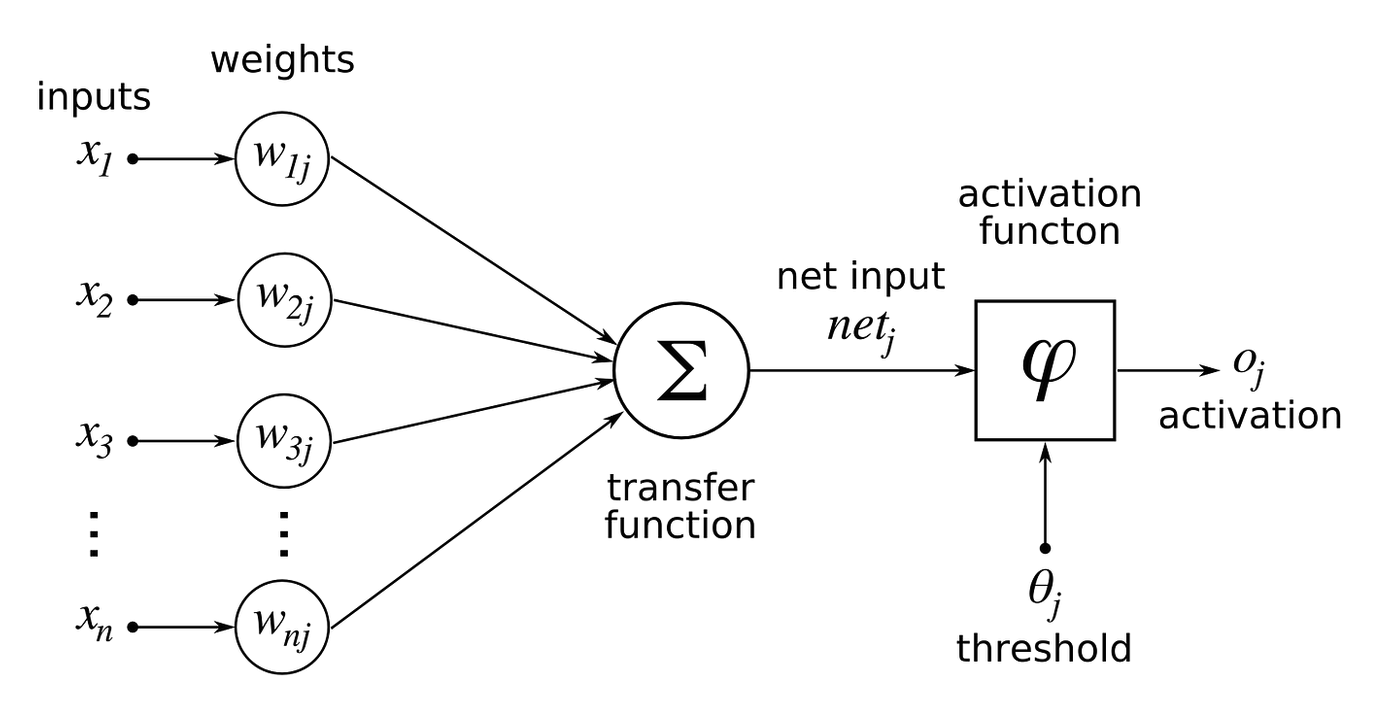
\includegraphics[width=\textwidth,height=0.72\textheight,keepaspectratio]{neuron.png}
\end{center}
\end{frame}

\begin{frame}{Single Hidden Layer Network}
\begin{itemize}
\item Input $x\in\mathbb{R}^{M}$, output $y\in\mathbb{R}^{N}$.

\item The $j$-th hidden unit:
\begin{equation}
h_{j}^{(1)} = f_{j}^{(1)}(x) = \sigma\!\left(b_{j}^{(1)}+\sum_{m=1}^{M}w_{j,m}^{(1)}x_{m}\right),\quad j=1,\dots,U_{1} \label{eq:hidden1}
\end{equation}

\item The $i$-th output:
\begin{equation}
y_{i} = \sum_{j=1}^{U_{1}}\tilde{w}_{i,j}\,h_{j}^{(1)}+\tilde{b}_{i},\quad i=1,\dots,N \label{eq:output1}
\end{equation}

\item $\sigma$ is a nonlinear activation function.

\medskip
\item Common choices: $\sigma(x)=\tanh(x)$, $\sigma(x)=\max(0,x)$ (ReLU), $\sigma(x)=\frac{1}{1+e^{-x}}$ (sigmoid).
\end{itemize}
\end{frame}

\begin{frame}{Two Hidden Layer Network}
\begin{itemize}
\item Take the linear combination of $h^{(1)}$ and pass through another activation:
\begin{equation}
h_{j}^{(2)} = \sigma\!\left(b_{j}^{(2)}+\sum_{k=1}^{U_{1}}w_{j,k}^{(2)}\,f_{k}^{(1)}(x)\right),\quad j=1,\dots,U_{2} \label{eq:hidden2}
\end{equation}
\begin{equation}
y_{i} = \sum_{j=1}^{U_{2}}\tilde{w}_{i,j}\,h_{j}^{(2)}+\tilde{b}_{i},\quad i=1,\dots,N \label{eq:output2}
\end{equation}

\medskip
\item \textbf{Pattern:} Each layer performs a linear transformation followed by a nonlinear activation. Depth adds representational power.

\medskip
\item \textbf{Macro analogy:} Successive layers are like successive time steps in a dynamic program --- each transforms the ``state'' into a richer representation.
\end{itemize}
\end{frame}

\begin{frame}{Hidden Layers: Visual}
\begin{center}
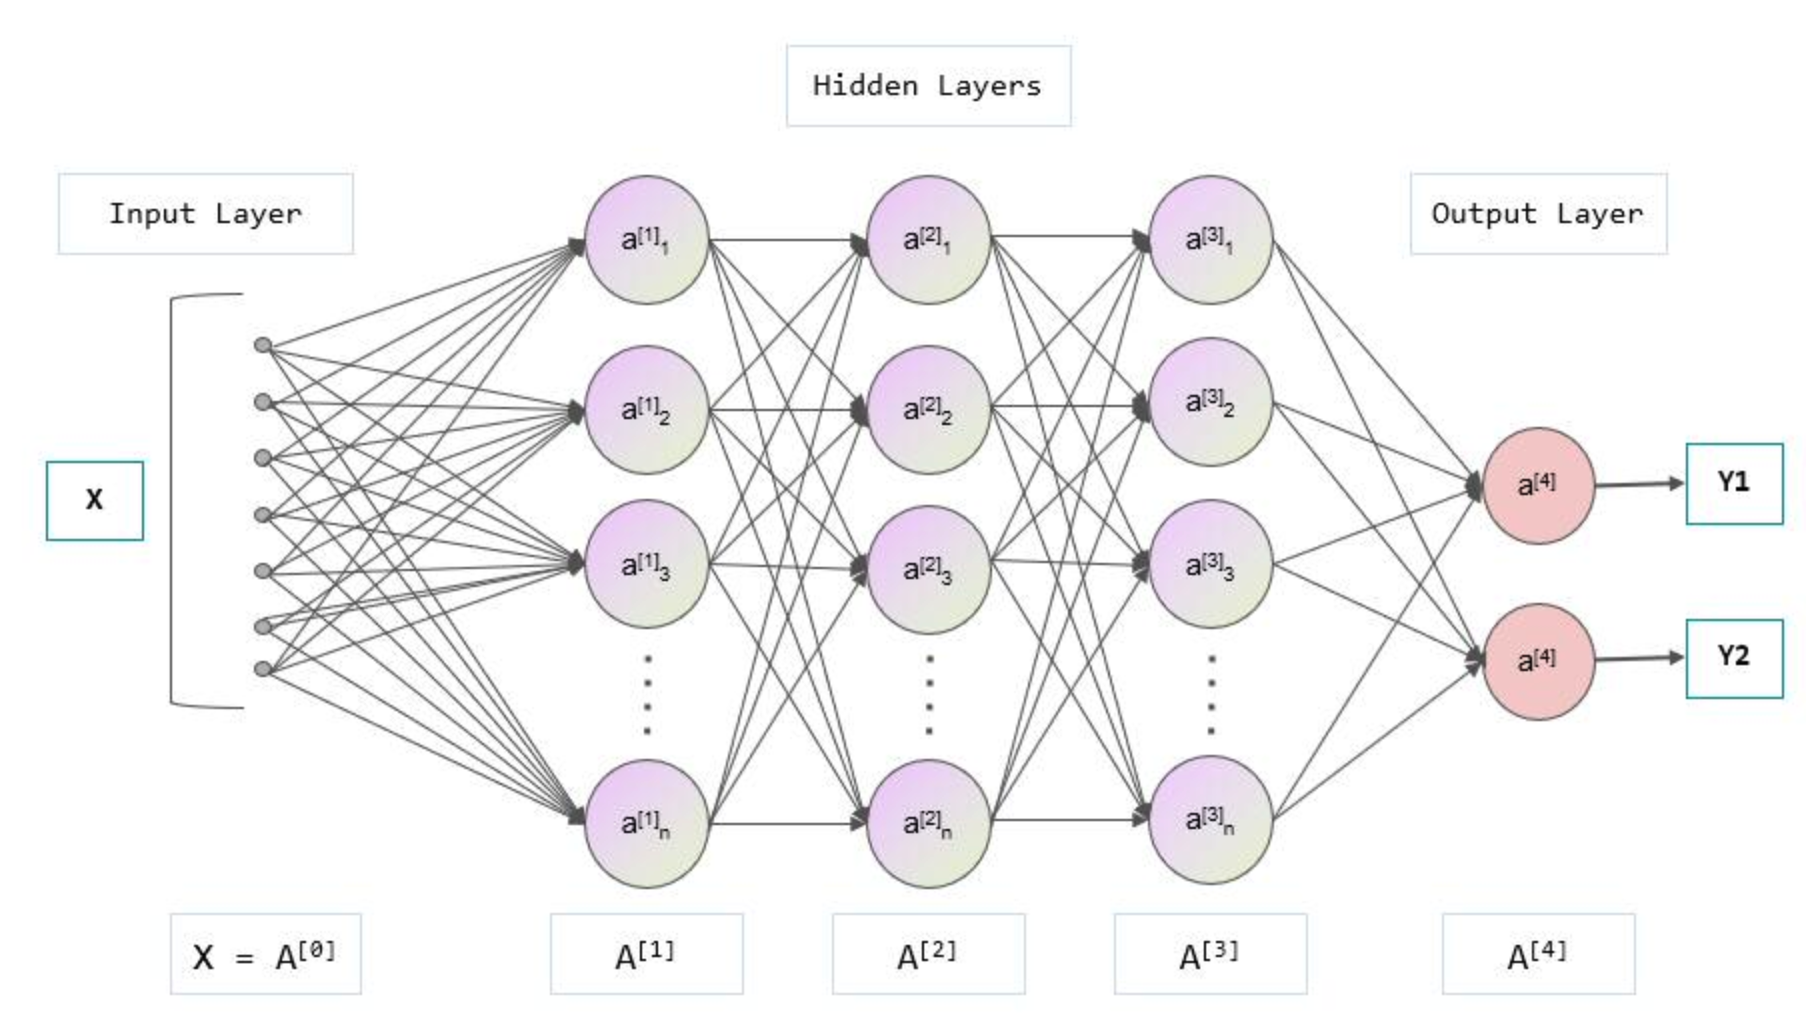
\includegraphics[width=12cm]{dnn}
\end{center}
\end{frame}

%=============================================================================
\section{Activation Functions and Universal Approximation}

\sectiondivider{Activation Functions and Universal Approximation}{Nonlinearity is the point: sigmoid, tanh, ReLU --- and why two layers approximate anything}

\begin{frame}{Activation Functions: Visual}
\begin{center}
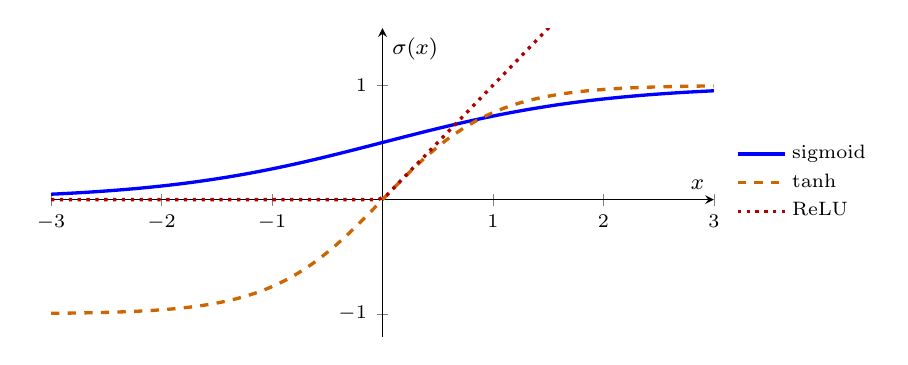
\begin{tikzpicture}
\begin{axis}[
    width=10cm, height=5.5cm,
    xmin=-3, xmax=3, ymin=-1.2, ymax=1.5,
    axis lines=middle,
    xlabel={$x$}, ylabel={$\sigma(x)$},
    tick label style={font=\scriptsize},
    label style={font=\footnotesize},
    legend style={font=\scriptsize, draw=none, at={(1.02,0.5)}, anchor=west},
    legend cell align=left,
    samples=80,
]
\addplot[blue, very thick, domain=-3:3] {1/(1+exp(-x))};
\addlegendentry{sigmoid}
\addplot[orange!80!black, very thick, dashed, domain=-3:3] {tanh(x)};
\addlegendentry{tanh}
\addplot[red!70!black, very thick, dotted, domain=-3:3] {max(0,x)};
\addlegendentry{ReLU}
\end{axis}
\end{tikzpicture}
\end{center}
\vspace{-2mm}
{\footnotesize\textit{Sigmoid \& tanh saturate ($\Rightarrow$ vanishing gradients); ReLU is piecewise linear ($\Rightarrow$ sparse activation, fast gradient flow).}}
\end{frame}

\begin{frame}{Activation Functions: What They Do}
\begin{itemize}
\item \textbf{Sigmoid:} $\sigma(x) = \frac{1}{1+e^{-x}}$ --- outputs in $(0,1)$, useful for probabilities.
\medskip
\item \textbf{Tanh:} $\tanh(x)$ --- outputs in $(-1,1)$, zero-centered, smoother than ReLU.
\medskip
\item \textbf{ReLU:} $\max(0,x)$ --- simple, sparse activation, dominant in modern networks.
\medskip
\item \textbf{Why nonlinearity matters:} without activation functions, stacked layers collapse into one linear map --- depth gains us nothing without nonlinearity.

\medskip
\item \textbf{For economists:} the activation is the network's analogue of choosing a flexible functional form (translog, CES, semi-parametric) --- but the network composes it across layers.
\end{itemize}
\end{frame}

\begin{frame}{Function Approximation with ReLU}
\begin{itemize}
    \item \textbf{Goal:} Approximate arbitrary nonlinear functions using simple building blocks.
    \item \textbf{Key Idea:} Linear combination of shifted ReLU functions:
    \[
    \hat{y}(x) = a_0 + \sum_{i=1}^{N} a_i\,\text{ReLU}(x-b_i)
    \]
    \item \textbf{Shifts $b_i$:} Define the ``kink'' points where marginal slope changes.
    \item \textbf{Coefficients $a_i$:} Scale each ReLU's contribution to match local slope.

    \medskip
    \item \textbf{Example:} Approximating $\sin(x)$ on $[-\pi, \pi]$:
    \begin{itemize}
        \item Choose shifts $b_i$ evenly over the domain
        \item Form design matrix with columns $\text{ReLU}(x-b_i)$ and a bias
        \item Solve a least-squares problem for coefficients $a_i$
    \end{itemize}

    \medskip
    \item \textbf{Economist's take:} ReLU kinks are piecewise-linear splines --- the network \emph{learns} the knot locations, unlike a fixed Chebyshev grid.
\end{itemize}
\end{frame}

\begin{frame}{ReLU Approximation: Increasing Complexity}
\begin{center}
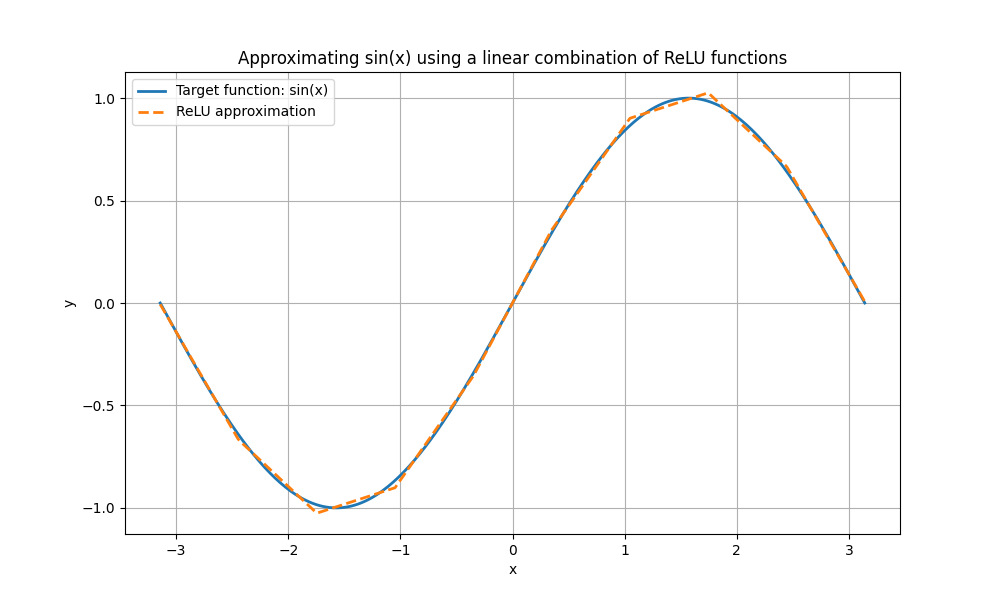
\includegraphics[width=12cm,height=7.5cm,keepaspectratio]{relu1}
\end{center}
\end{frame}

\begin{frame}{ReLU Approximation: More Kink Points}
\begin{center}
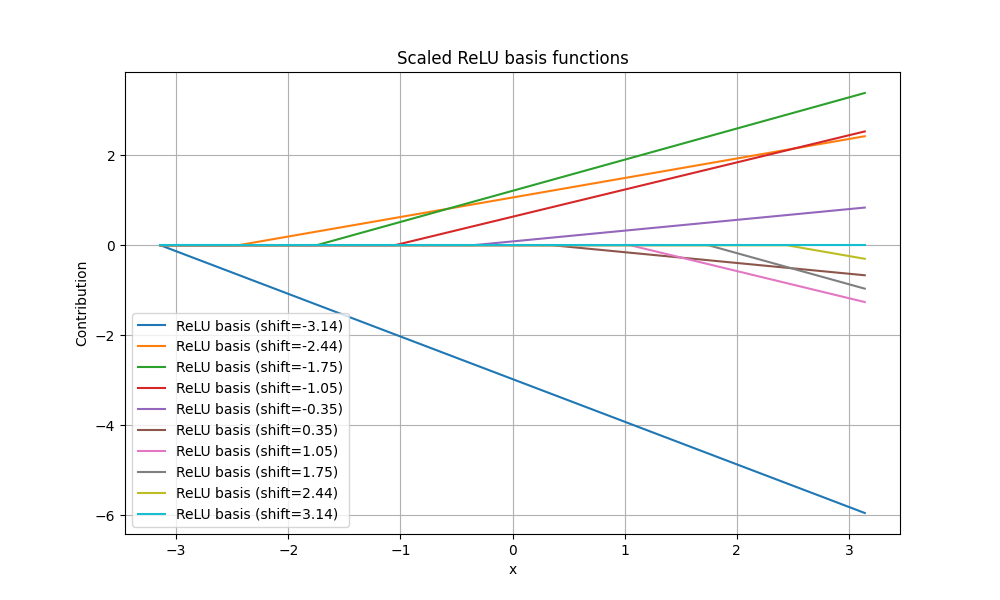
\includegraphics[width=12cm,height=7.5cm,keepaspectratio]{relu2}
\end{center}
\end{frame}

\begin{frame}{ReLU Approximation: High Fidelity}
\begin{center}
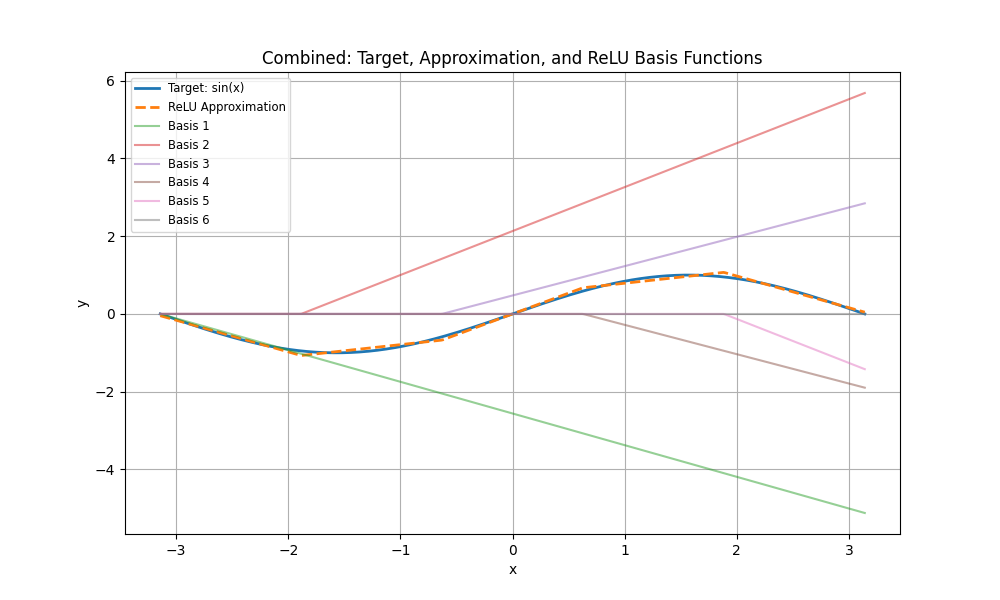
\includegraphics[width=12cm,height=7.5cm,keepaspectratio]{relu3}
\end{center}
\end{frame}

\begin{frame}{Why Neural Networks Work: Universal Approximation}
\begin{tcolorbox}[colback=blue!3, colframe=blue!40, title={Universal Approximation Theorem (Cybenko 1989; Hornik 1991)}]
\small Any continuous function on $[0,1]^d$ can be approximated \emph{uniformly} by a two-layer network --- for sigmoidal $\sigma$ (Cybenko), for any bounded nonconstant $\sigma$ (Hornik), indeed for \emph{any} non-polynomial $\sigma$ (Leshno, Lin, Pinkus \& Schocken 1993).
\end{tcolorbox}
\smallskip
\begin{conceptbox}
\small\textbf{Intuition --- you just watched the proof.} Those ReLU plots \emph{were} the construction: a weighted sum of shifted kinks $\sum_i a_i\,\mathrm{ReLU}(x-b_i)$ bends to fit any curve, and a sigmoid network stacks soft ``bumps'' the same way. \textbf{One hidden unit $=$ one building block; add units $\Rightarrow$ shrink the error.} Nonlinearity is the glue --- drop it and the whole sum collapses back to a single straight line.
\end{conceptbox}
\smallskip
\begin{cautionbox}
\small\textbf{Existence, not a recipe.} UAT promises a good network \emph{exists} --- not that training will \emph{find} it, nor that ``enough'' units is a \emph{small} number. Approximation $\neq$ optimization $\neq$ generalization; T3 takes on the finding. \emph{(The same theorem later is why transformer attention approximates --- Lec.\ 7.)}
\end{cautionbox}
\end{frame}

\begin{frame}{Why Neural Networks Work: Beating the Curse of Dimensionality}
\begin{tcolorbox}[colback=green!3, colframe=green!40, title={Barron (1993): a dimension-free rate}]
\small A one-hidden-layer network reaches squared error of order $O(1/M)$ in $M$ units --- \emph{independent of the input dimension $N$}. Fixed series bases (polynomials, splines, Chebyshev) manage only $O(1/M^{2/N})$: to hold accuracy as $N$ grows, $M$ must blow up exponentially.
\end{tcolorbox}
\vspace{-2mm}
\begin{columns}[T]
\column{0.58\textwidth}
\small\textbf{Why the gap?}
\begin{itemize}\small\setlength\itemsep{2pt}
    \item \textbf{Grid basis is fixed:} resolution $k$ per axis needs $k^{N}$ pieces --- most parked where $f$ barely moves. That is the curse.
    \item \textbf{A neuron is a ridge $\sigma(w^\top x+b)$:} a soft step aimed along a \emph{learned} direction $w$. The net spends its $M$ units where $f$ varies --- so error tracks $f$'s \emph{intrinsic} complexity, not the dimension $N$.
\end{itemize}
\column{0.42\textwidth}
\begin{center}
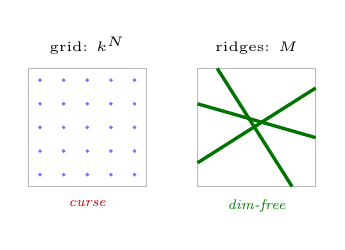
\begin{tikzpicture}[font=\tiny]
  % series: fixed tensor grid --- many points
  \draw[gray!55] (0,0) rectangle (1.5,1.5);
  \foreach \i in {0,...,4}\foreach \j in {0,...,4}
     \fill[blue!55] (0.15+\i*0.3,0.15+\j*0.3) circle (0.025);
  \node[anchor=south] at (0.75,1.55) {grid: $k^{N}$};
  \node[red!70!black,anchor=north,font=\tiny\itshape] at (0.75,-0.05) {curse};
  % network: few learned ridge directions
  \begin{scope}[shift={(2.15,0)}]
    \draw[gray!55] (0,0) rectangle (1.5,1.5);
    \draw[green!45!black,very thick] (0,0.30)--(1.5,1.25);
    \draw[green!45!black,very thick] (0.25,1.5)--(1.20,0);
    \draw[green!45!black,very thick] (0,1.05)--(1.5,0.62);
    \node[anchor=south] at (0.75,1.55) {ridges: $M$};
    \node[green!45!black,anchor=north,font=\tiny\itshape] at (0.75,-0.05) {dim-free};
  \end{scope}
\end{tikzpicture}
\end{center}
\end{columns}
\vspace{-2mm}
\begin{takeawaybox}\small
\textbf{For economists:} this is why deep learning cracks high-dimensional dynamic models --- heterogeneous-agent macro, many assets and shocks --- exactly where Chebyshev and tensor grids break down (Lec.\ 4--6; the DeepRamsey case).
\end{takeawaybox}
\end{frame}

\begin{frame}{DNN = Linear Transformation + Nonlinear Activation}
\begin{itemize}
\item \textbf{Linear Transformation:}
\begin{itemize}
\item Each neuron performs a weighted sum of inputs: projects data onto a new axis
\item The set of transformations across a layer creates a \emph{new representation}
\item Enables: flexible feature representation, information compression, interaction capture
\end{itemize}

\medskip
\item \textbf{Nonlinear Activation:}
\begin{itemize}
\item Allows the network to capture nonlinearity and complex patterns
\item Creates curved decision boundaries in the feature space
\item \textbf{Essential} for the universal approximation property
\end{itemize}

\medskip
\item \textbf{Together:} Each layer applies an affine map $Wx+b$ then a pointwise nonlinearity $\sigma(\cdot)$. Stacking layers composes these maps:
\[
f(x) = \sigma_L \circ A_L \circ \cdots \circ \sigma_1 \circ A_1 (x)
\]
where $A_\ell(x) = W_\ell x + b_\ell$.

\end{itemize}
\end{frame}

%=============================================================================
% House-style bridge closer (matches Lec05/Lec09): restate the act, hand off.
\begin{frame}{Bridge: A Good Network \emph{Exists} --- Now We Must \emph{Find} It}
\textbf{Act 3.2 built the object. A network is a composition of affine maps and pointwise nonlinearities; universal approximation says a good one \emph{exists}, and Barron says width buys accuracy at a rate the input dimension cannot destroy.}

\vspace{0.25cm}
\begin{itemize}
  \item You have seen \emph{what}: neurons, layers, and activations --- and why nonlinearity is essential (drop it and the whole stack collapses to one straight line).
  \item \textbf{Next (3.3):} existence is not a recipe. The finding machinery --- forward pass, backpropagation, stochastic gradient descent --- plus the regularization discipline that keeps the fit honest.
\end{itemize}

\vspace{0.3cm}
\begin{center}
\footnotesize\textit{Arc: 3.1 WHY (the case for ML) $\;\to\;$ \textbf{3.2 BUILD} (architecture $+$ UAT) $\;\to\;$ 3.3 TRAIN (backprop $+$ SGD) $\;\to\;$ 3.4 SHAPE (economics-aware nets $+$ lab).}
\end{center}
\end{frame}

\end{document}
